\section{Phonemes}
\label{SBN}
In order to articulate the percussive vocal sounds in terminologies this study revealed mainly two important ways to do so, the International Phonetic Alphabet (IPA) \citep{ipa} and the Standard Beatboxing Notation (SBN), which are also briefly described in this chapter \\footnote{\url{www.humanbeatbox.com/forum/content.php/370-Standard-Beatbox-Notation}}.


Sounds can be described as phonemes. Although phonemes are not a focus of this project, it is still important to remember that beatboxing can be a complex artform, and one would need a comprehensive systematic approach which could be somewhat facilitated by understanding and utilizing aspects of the IPA, the SBN, or a combination of both.


We found the most relevant articulation of phonemes for this project to be the SBN, as it is actually based on a “simplified” approach to the IPA. The technical characteristics of the phonemes used for notations is the way to describe the sounds used in beatboxing, which have much in common with the IPA. \\


The four types of phonetic sounds in beatboxing \citep{BeatboxBible}:

  \begin{itemize} 
	\item\textbf{Plosives}

	
	Plosives are sounds where one stop the airway and release sound. Often used for kicks and snares.
  
	\item\textbf{Fricatives}
	
	
	{Fricatives are continuous sounds like “schhh”, “tsss”. Often used to imitate cymbals.}
	
	\item\textbf{Clicks}
	
	
	{Clicks are more subtle sounds that are often used to imitate claps and snaps, but also subtle snares.}
	
	\item\textbf{Oscillations}
	
	{Oscillations sounds are continuous sounds imitating synthesized instruments and robotic sounds like vibratos and alarms.}
\end{itemize}

Each of these four groups of sounds can be described into further detailed characteristics and potential utilizability in transcription of beatboxing, but the main purpose of this chapter is mainly to get acquainted with the techniques and articulations of the beatboxing sounds, and an idea of the phonetic complexity. This information could be useful when taking further steps towards the development of a complex transcription of beatboxing.
%\begin{figure}[h]
%	\begin{center}
%		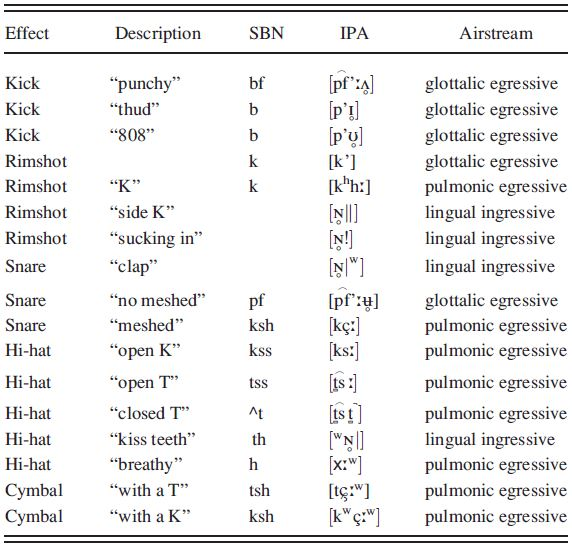
\includegraphics[height=5cm]{fig/phonemes.JPG}
%		\caption{Illustration of phonemes utilized in Michael Proctors study on beatboxing \citep{proctor2012}}
%		\label{VoiceBand}
%	\end{center}
%\end{figure}
